\appendix
\chapter{Weitere Abbildungen und Tabellen}
\label{appendix:abb_tab}
\begin{figure}[h!]
    \centering
    
\includegraphics[scale=10]{images/2-1_chroma_artefacts_original.png}
    
\includegraphics[scale=10]{images/2-1_chroma_artefacts_sampled.png}
    \caption{Artefakte durch Chroma Subsampling}
    \textit{Links: Original, Rechts: Subsampled. Die rechte Kante des blauen Farbblocks liegt in gesubsampleten 2x2 Blöcken, wodurch Artefakte entstehen. Die linke Kante liegt zwischen zwei 2x2 Blöcken, weshalb es zu keiner falschen Darstellung kommt.}
    \label{fig:chroma_artefacts}
\end{figure}

\begin{figure}[h!]
    \centering
    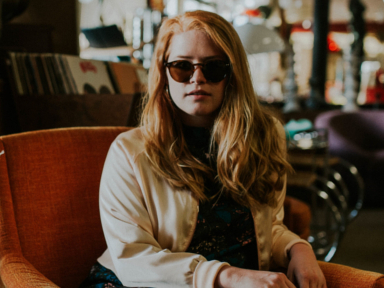
\includegraphics[scale=0.58]{images/2-3_brook_orig.png}
    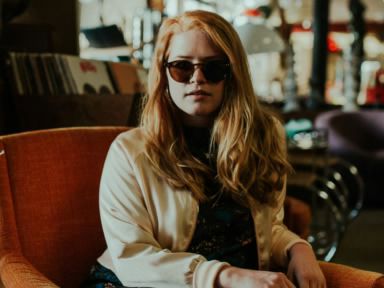
\includegraphics[scale=0.58]{images/2-3_brook_1.png}
    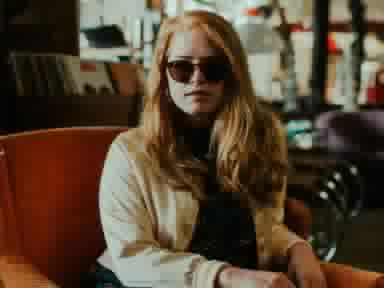
\includegraphics[scale=0.58]{images/2-3_brook_16.png}
    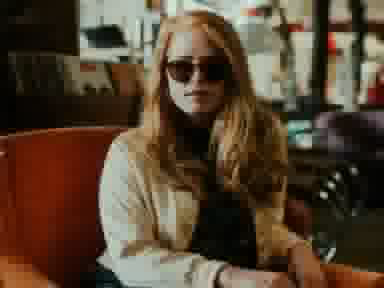
\includegraphics[scale=0.58]{images/2-3_brook_31.png}
    \caption{Ergebnis der Quantisierung mit verschiedenen Quantisierungsfaktoren}
    \textit{Oben links: Original, Oben rechts: Quantisiert mit Faktor 1, Unten links: Quantisiert mit Faktor 16, Unten rechts: Quantisiert mit Faktor 31.\\
    Mit zunehmendem Quantisierungsfaktor ist ein ansteigender Verlust der Bildqualität zu beobachten, wobei grobe Strukturen weitestgehend erhalten bleiben. Original nach \cite{brooke_cagle__2016}}
    \label{fig:quantization_multi_mquants}
\end{figure}

\begin{table}[h!]
\centering
\begin{tabular}{|c|c|c|c|c|c|c|c|}
	\hline
	8 & 16 & 19 & 22 & 26 & 27 & 29 & 34 \\
	16 & 16 & 22 & 24 & 27 & 29 & 34 & 37 \\
	19 & 22 & 26 & 27 & 29 & 34 & 34 & 38 \\
	22 & 22 & 26 & 27 & 29 & 34 & 37 & 40 \\
	22 & 26 & 27 & 29 & 32 & 35 & 40 & 48 \\
	26 & 27 & 29 & 32 & 35 & 40 & 48 & 58 \\
	26 & 27 & 29 & 34 & 38 & 46 & 56 & 69 \\
	27 & 29 & 35 & 38 & 46 & 56 & 69 & 83 \\
	\hline
\end{tabular}
\caption{Voreingestellte MPEG-1 Intracoding Quantisierungsmatrix. \cite{symes_peter_digital_2004} }
\label{tab:default_quant}
\end{table}

\begin{table}
\centering
\begin{tabular}{|ccc|l|l|}
	\hline
	\multicolumn{3}{|c|}{Genutzte Optionen}               & Größe in Kilobyte & Ratio \\
	RLE & Chroma Subsampling & Quantisierung mit Faktor &                   &       \\
	\hline
	X   &                    & -                        & 258.38            & 3.76  \\
	X   & X                  & -                        & 145.95            & 6.66  \\
	X   & X                  & 1                        & 58.32             & 16.67 \\
	X   & X                  & 16                       & 18.59             & 52.29 \\
	X   & X                  & 31                       & 16.23             & 59.89 \\
	\hline
\end{tabular}
\caption{Testergebnisse der angewandten Kompressionsalgorithmen}
\label{tab:test}
\end{table}


\begin{figure}[h!]
    \centering
   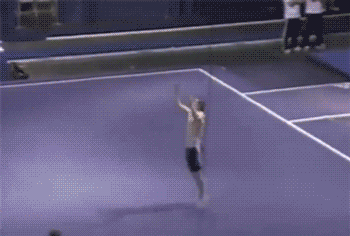
\includegraphics[scale=0.5]{images/corruptedGif/frame7.png}
    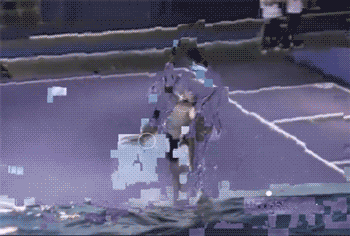
\includegraphics[scale=0.5]{images/corruptedGif/frame10.png}
    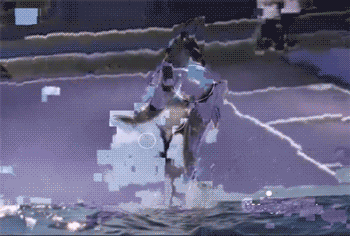
\includegraphics[scale=0.5]{images/corruptedGif/frame13.png}
        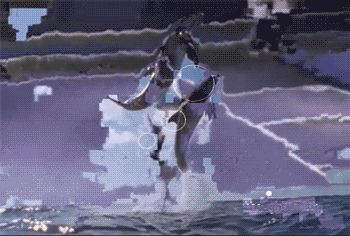
\includegraphics[scale=0.5]{images/corruptedGif/frame16.png}
            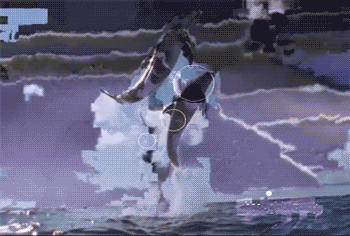
\includegraphics[scale=0.5]{images/corruptedGif/frame19.png}
                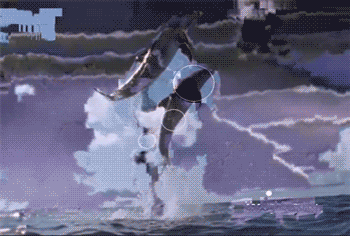
\includegraphics[scale=0.5]{images/corruptedGif/frame22.png}
    \caption{Bildartefakte beim Auslassen eines I-Frames}
    \textit{Es wird jeder dritte Frame eines GIFs gezeigt, welches einen Szenenwechsel von einem Turner hinzu zu zwei springendem Delfinen darstellt. Hierbei wurde im Ursprungsvideo mit Absicht der beim Szenenwechsel erzeugte I-Frame zerstört um künstlich Bildartefakte zu erzwingen und sogenannte \glqq{Glitch-Art} zu erzeugen.}
    \linebreak
    Quelle: In Einzelbilder aufgeteiltes GIF nach: http://forum.glitchet.com/t/tutorial-make-video-glitch-art-how-to-datamosh-in-plain-english/36
    \linebreak Zuletzt abgerufen am 13.12.2016
\end{figure}

\begin{figure}[h!]
    \centering
    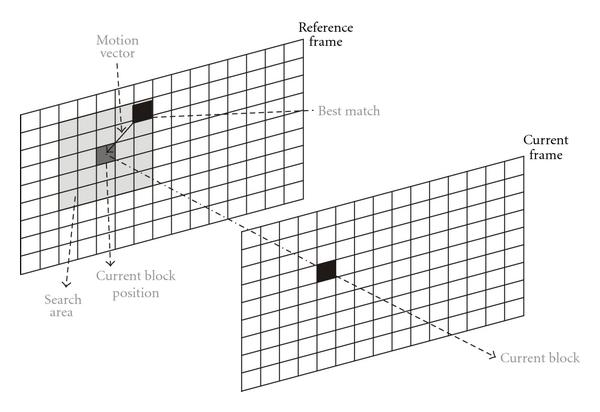
\includegraphics[scale=3]{images/3-2-3_motionCompensation.jpg}
    \caption{Suchen von identischen Blöcken in zwei Frames mittels Bewegungskorrektur}
    \textit{Das Referenz Bild wird anschließend mit dem resultierenden Motion Vektor codiert}
    Quelle: \cite{lopes_memory_2012}
\end{figure}

\chapter{Listings}

\lstinputlisting[language=Python, caption=Implementierung der DCT für ein 8x8 Array, label=lst:impl_dct]{snippets/dct.py}
\newpage
\lstinputlisting[language=Python, caption=Implementierung des Quantisierungsprozesses nach MPEG-1 Standard ohne Clipping, label=lst:quantizer]{snippets/quantizer.py}

\chapter{Erläuterung des Testvorgehens}
\label{chap:testvorgenen}

Als Grundlage der Testvorgänge diente das dieser Arbeit auf CD beiliegende Programm. Das Chroma Subsampling ist als Mittelwertberechnung von jeweils 2x2 Blöcken während der Kompression realisiert. Die DCT ist wie im Kapitel \ref{chap:dct} vorgestellt implementiert. Als Quantisierungsmatrix wird die in Tabelle \ref{tab:default_quant} dargestellte MPEG-1 Intracoding Quantisierungsmatrix verwendet. Das Verfahren ist nach Listing \ref{lst:quantizer} implementiert. Als Lauflängencodierung wird eine abgewandelte Form des ZigZag Encodings nach JPEG-Standard verwendet. Hierbei werden lediglich Nullen lauflängencodiert, was in der Praxis ein Symbol für die Angabe des RLE encodierten Zeichens spart. Aufgrund der Charakteristik der aus der Quantisierung resultierenden Matrix hat sich diese Form als effizienter herausgestellt, als eine klassische RLE. Da kein Predictive Coding der DC-Werte verwendet wird, werden, anders als im JPEG Standard, auch diese Werte encodiert. Zur Berechnung der resultierenden Bildgrößen wurden folgende Werte angenommen: Jeder RGB Kanal lässt sich als 8 Bit Integer darstellen. Da jedes Pixel aus drei RGB Kanälen besteht resultiert hieraus eine Größe von 24 Bit. Zur Speicherung der Werte eines RLE encodierten Deskriptors werden aufgrund der zusätzlich benötigten Symbole jeweils 9 Bit benötigt. Als Quellbild wurde das in \ref{fig:quantization_multi_mquants} dargestellte Originalbild verwendet. Die Speicherung der RGB Werte benötigt nach oben beschriebener Annahme 324 Kilobyte. Das Bild hat eine Abmessung von 288x384 Pixel.

